\documentclass[12pt,a4paper]{article}
\usepackage[utf8]{inputenc}
\usepackage[czech]{babel}
\usepackage[T1]{fontenc}
\usepackage[export]{adjustbox}
\usepackage{graphicx}
\usepackage{listings}
\usepackage{pdfpages}
\usepackage{float}

\begin{document}
%
%	TITLE
%
\begin{titlepage}
	
\includegraphics[left]{images/logo_fav}\par
	\vspace{5cm}
	{
		\centering
		\Huge{\textbf{Nápojový automat}}\\
		\Huge{\textbf{\textit{KIV/TI - Semestrání práce}}}\\
	}	
	\vfill
    \begin{tabular}{ll}
		vypracovali: & \it{Martin Matas, Martin Formánek, Tomáš Dubina} \\
		%studijní číslo: & A15B0089P \\
		%email: & martinm@students.zcu.cz \\
		datum: & {\large 27. listopadu 2016\par}
	\end{tabular}
\end{titlepage}
%
%	OBSAH
%
\tableofcontents
\newpage
%
%	TEXT
%
\section{Zadání}

\paragraph{\parindent=4em}{
	Vytvořte konečný automat pro řízení nápojového automatu. Automat bude mít tři typy vstupů: stisky tlačítek, indikaci hodnoty vhozené mince a signály z různých čidel (např. "došla káva", "došly kelímky" aj.). Svými výstupy bude automat řídit motory, elektromagnety apod., které zajistí vracení mincí z mincovníku, přípravu kelímku, ohřívání vody, napouštění vody apod. Konkrétní vnitřní prvky automatu si realisticky navrhněte sami.
}

\paragraph{\parindent=4em}{	
	Vytvořte dále aplikaci, která vhodným způsobem simuluje automat a umožňuje mačkání tlačítek, vhazování mincí a sledování vrácení přeplatku, rovněž by měla umožnit simulovat výjimečné stavy, např. "neteče voda" apod.
Hlavním smyslem zadání je vyzkoušet si návrh implementace pomocí konečného automatu.
}

\section{Teoretický rozbor}

\paragraph{\parindent=4em}{	
	Nápojový automat by měl zákazníkovi umožnit vhození mincí, nastavení množství cukru a volbu nápoje. Po objednání zvoleného nápoje musí automat vrátit případný přeplatek zákazníkovi. Automat by měl mít ošetřené vstupy před vhozením nepodporovaných mincí. Měl by nabízet pouze nápoje, ke kterým má všechny potřebné přísady, v případě, kdy automat nemá
	přísady pro přípravu nápoje, uvede se do stavu {\it Mimo provoz}. Pokud by došlo k výjimečnému stavu (např. odpojení přívodu s vodou), měl by automat umožnit zákazníkovi stornovat objednávku a vrátit peníze.
}

\newpage
\section{Teoretické řešení}

\begin{figure}[H]	
	\centering
	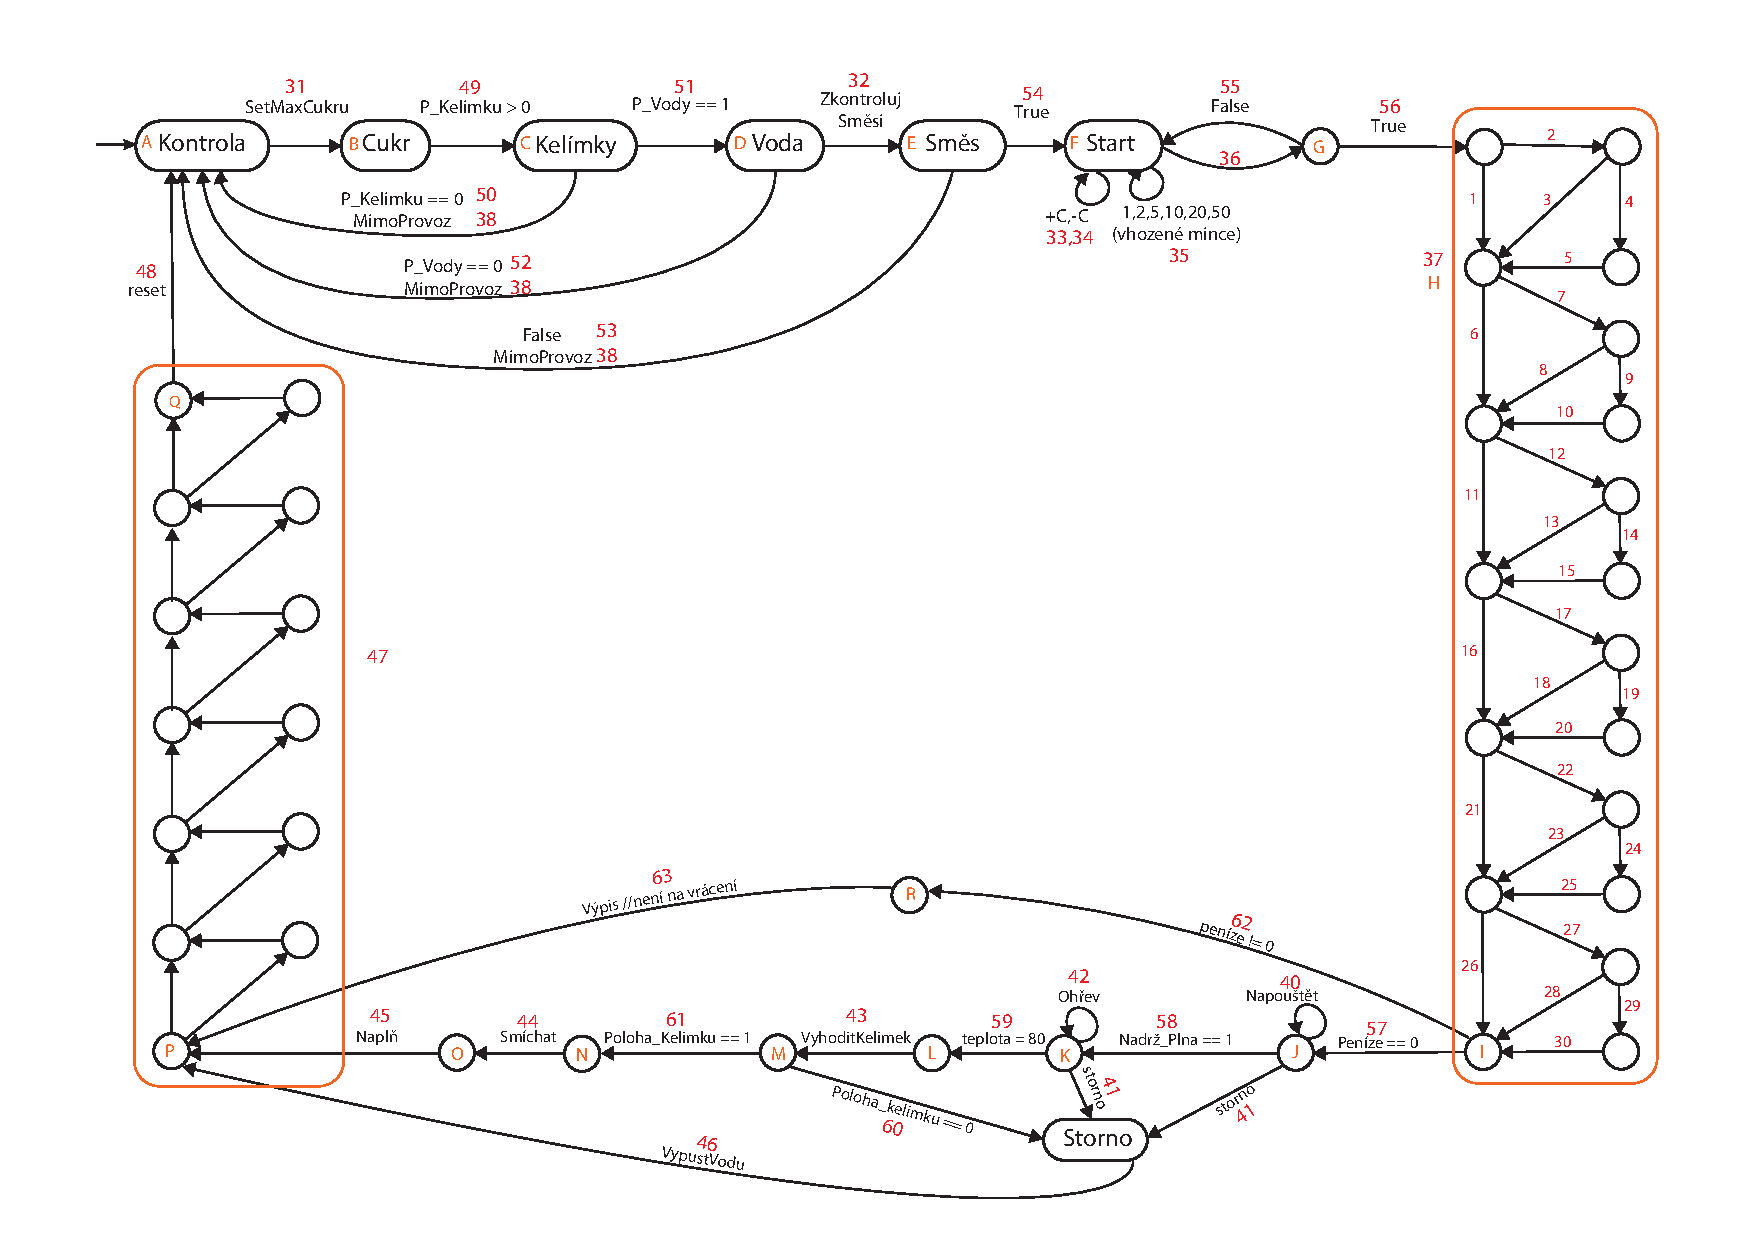
\includegraphics[angle=-90,width=\textwidth]{doc/kavovar_KA.pdf}
	\caption{Nákres konečného automatu}
\end{figure}
	
\paragraph{\parindent=4em}{	
	Stavy mezi H a I zajišťují převedení přeplatku na mince, které má automat k dispozici. Nejprve se testuje, jestli lze přeplatek vrátit v mincích hodnoty 50 Kč, pokud je to možné, automat spočte, kolik takových mincí může vrátit. Poté odečte částku, kterou vrátí v těchto mincích od celkového přeplatku a pokračuje mincemi hodnoty 20 Kč. Pokud automat nemůže částku vrátit v mincích hodnoty 50 Kč, přejde rovnou na mince hodnoty 20 Kč a takto pokračuje až po hodnotu 1 Kč. Pokud nastane situace, že automat dojde do stavu I a přeplatek nebude 0 Kč, automat nemá na vrácení a přejde do stavu, kdy vrátí uživateli vhozenou částku.
}	

\paragraph{\parindent=4em}{	
	Stavy mezi P a Q zajišťují vrácení přeplatku. O to, které mince musí automat zákazníkovi vrátit se starají stavy mezi stavem H a I. Mechanismus je podobný tomu, který zjišťuje jaké mince vrátit. Nejprve automat testuje, jestli má nějaké mince hodnoty 50 Kč k vrácení, pokud ano, vrátí zákazníkovi vypočtený počet mincí této hodnoty, poté přejde na mince hodnoty 20 Kč. Když automat nemá vracet žádné mince hodnoty 50 Kč, zkusí jestli má vrátit mince hodnoty 20 Kč atd..
}	

\begin{figure}[H]	
	\centering
	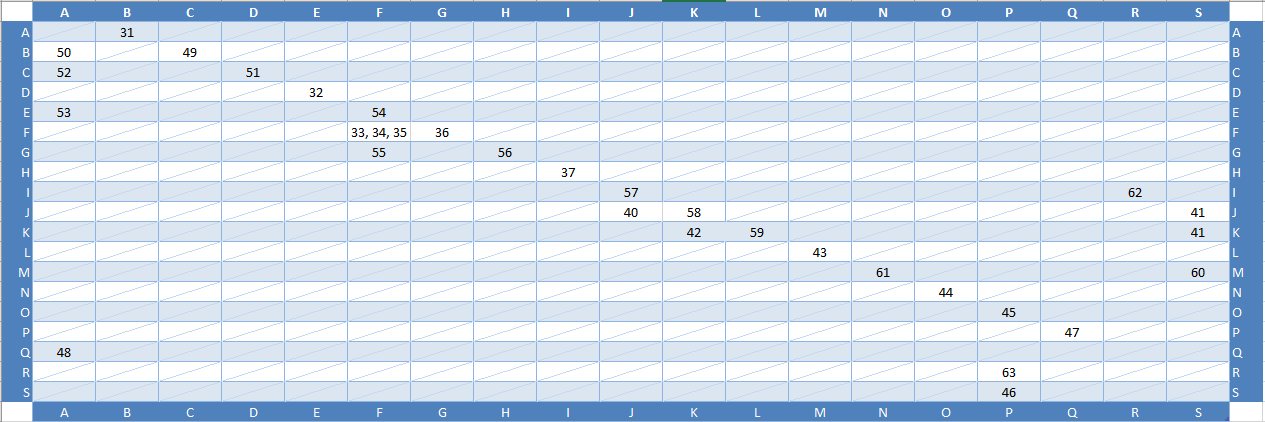
\includegraphics[width=\textwidth]{images/tabulka_prechodovych_funkci}
	\caption{Tabulka přechodových funkcí KA}
\end{figure}

\section{Implementace}

\paragraph{\parindent=4em}{	
	Nápojový automat je implementován v jazyce Java. Celá aplikace funguje v konzolovém režimu. V hlavním konstruktoru se nastaví všechny důležité parametry pro chod automatu např. přísun vody, počet kelímků, počet nápojových směsí atd. V aplikační třídě se tedy vytvoří instance tohoto automatu a nad touto instancí zavoláme metodu {\it startKA()} na spuštění automatu. V této metodě si nastavíme proměnnou {\it stav} na výchozí stav {\it A}. Dále metoda pokračuje do cyklu {\it while}, v kterém je {\it switch}, který přepíná mezi stavy. Ve stavu {\it F} očekáváme vstup od uživatele. Ze stavu {\it Q} se automat znovu přepne do výchozího stavu {\it A}.
}

\section{Struktura adresáře}

\begin{figure}[H]	
	\centering
	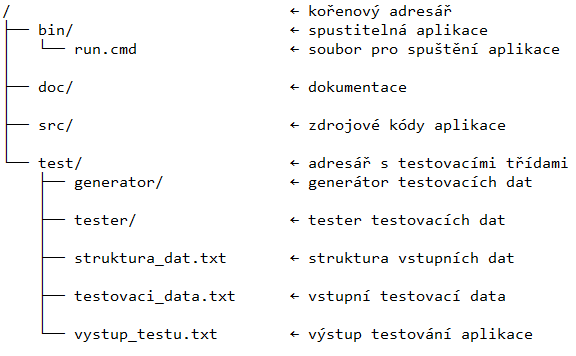
\includegraphics[width=\textwidth]{images/adresar}
	\caption{Adresářová struktura}
\end{figure}

\section{Uživatelská příručka}

\subsection{Spuštění aplikace}

\paragraph{\parindent=4em}{	
	Aplikace se spouští souborem {\it run.cmd} v adresáři {\it bin}.
}

\subsection{Po spuštění}

\paragraph{\parindent=4em}{	
	Po spuštění aplikace se uživateli zobrazí stručný návod jak aplikaci používat viz obr. \ref{fig:pospusteni}.
}

\begin{figure}[H]	
	\centering
	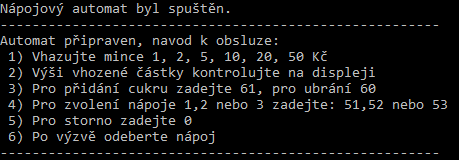
\includegraphics[width=\textwidth]{images/spusteni}
	\caption{Stručný návod po spuštění}
	\label{fig:pospusteni}
\end{figure}

\subsection{Ovládání}

\paragraph{\parindent=4em}{	
	Aplikace se ovládá pomocí klávesnice, zadáním příslušného vstupu pro operaci.
}

\section{Závěr}

\paragraph{\parindent=4em}{	
	Podle zadání jsme vytvořili návrh konečného automatu pro nápojový automat, který jsme posléze implementovali jako konzolovou aplikaci. Při vytváření aplikace vznikly nesrovnalosti mezi návrhem konečného automatu a implementací z důvodu jednoduššího zapsání algoritmu pro vracení přeplatku. Dále jsme museli pozměnit chod automatu, kvůli zautomatizování testování aplikace.
}

%
%	KONEC
%
\end{document}